\documentclass[12pt,a4paper,oneside]{article}

\usepackage{graphicx}
\usepackage{amsmath}

\begin{document}

\begin{titlepage}

\centering
	
\includegraphics[width=4cm]{logo.jpg}
	\vfill
    {\bfseries\Large
        DT2118 Lab2: Hidden Markov Models with Gaussian Emissions
        \vskip1cm
        Thomai Stathopoulou\\
        \vskip1cm
        April 30th, 2015
    }    
   \vfill
\end{titlepage}

\section{Multivariate Gaussian Density}
The goal of the second Lab is to implement and test different methods for isolated word recognition. We use the utterances used for the first Lab and the computed MFCC features.

The function ``log\_multivariate\_normal\_density\_diag'' computes:

\begin{equation}
log\_emlik[i, j] = log\phi_j(x_i) = log\mathcal{N}(x_i, \mu_j, \Sigma_j) = logP(x_i | \mu_j, \Sigma_j)
\end{equation}

In the case of a Gaussian Mixture Model (GMM) this is the log likelihood of each observation $x_i$ (each frame of an utterance signal)and each Gaussian distribution. In the case of a Hidden Markov Model (HMM) it is the emission probability of each observation and each state of the HMM.

Figures \ref{fig:gmm_obsloglik} and \ref{fig:hmm_obsloglik} show the log likelihoods as were calculated and as were expected.


\begin{figure}[h]
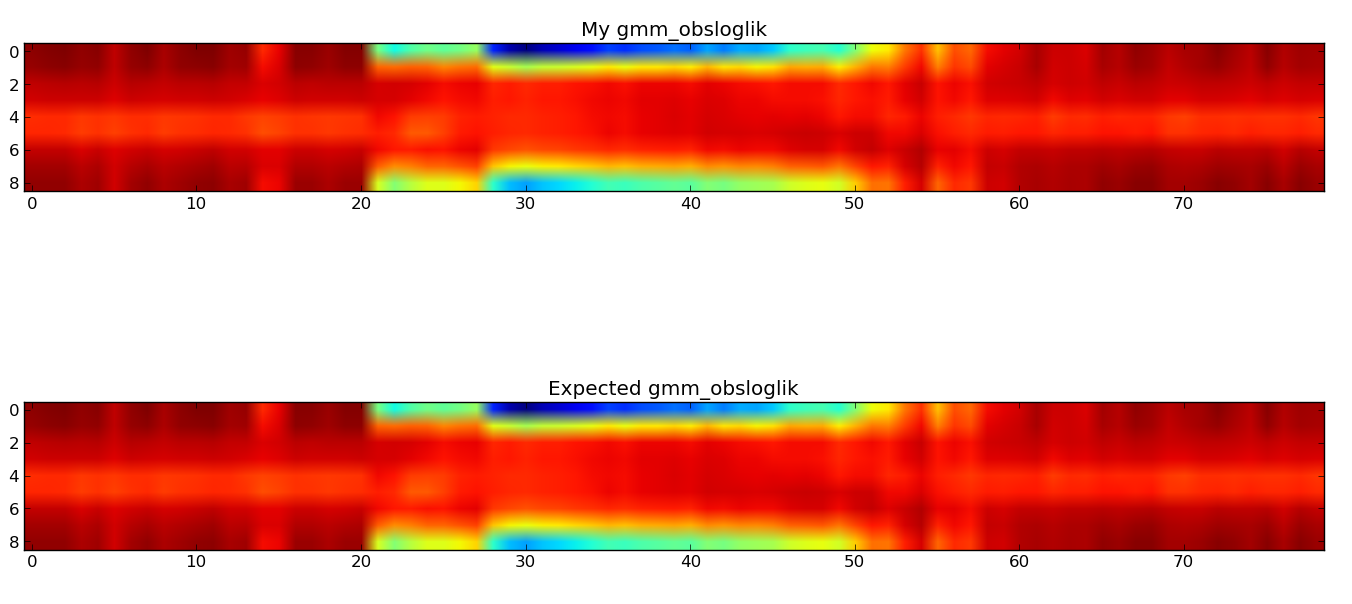
\includegraphics[scale=0.4]{../gmm_obsloglik.png}
\caption{Log likelihoods for every observation and every Gaussian Model}
\label{fig:gmm_obsloglik}
\end{figure}

\begin{figure}
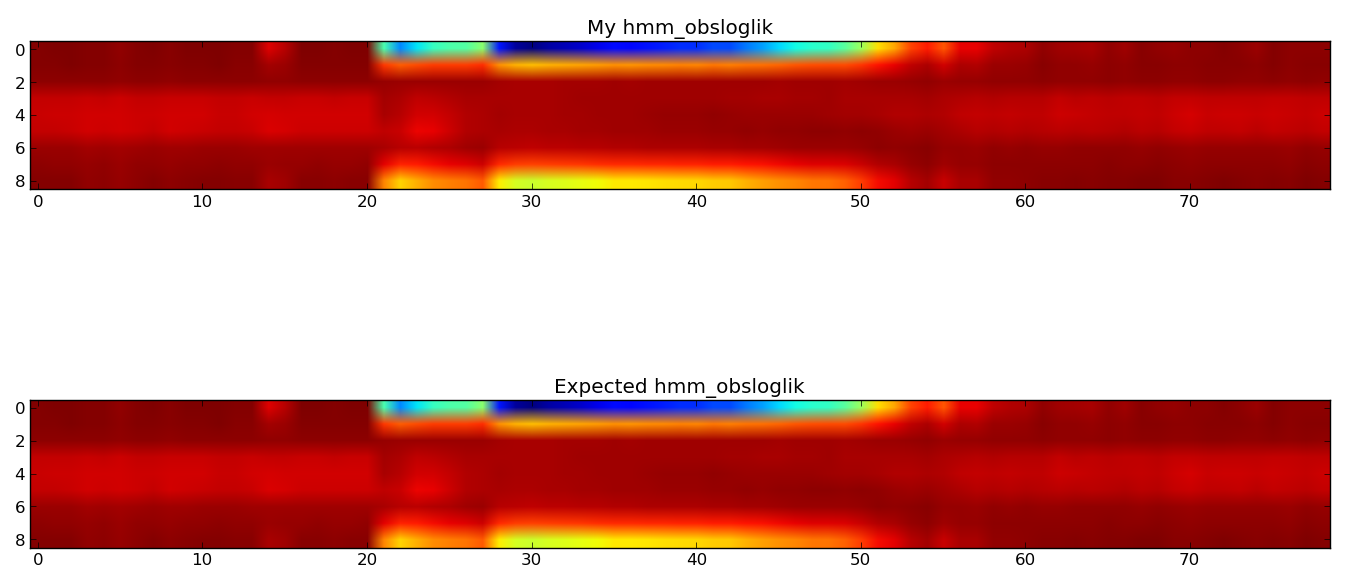
\includegraphics[scale=0.4]{../hmm_obsloglik.png}
\caption{Emission probabilities for every observation and every state of the HMM}
\label{fig:hmm_obsloglik}
\end{figure}

\section{GMM Likelihood and Recognition}
The function ``gmmloglik'' calculates the log likelihood of a sequence of observations (one utterance) for a specific GMM. That is, how probable it is that the sequence of observations is produced by a specific model. Since we are equipped with eleven models, each one of them trained on the utterances ``o'', ``zero'', ``one'' etc., by calculating the likelihood of every utterance for every model, we basically calculate the probability, that an utterance is indeed the digit of the corresponding model.

After calculating the ``gmm\_loglik'' of every utterance in the ``tidigits'' dataset for every model, for each utterance, we choose the model with the highest likelihood and we assign its digit to the utterance. Table \ref{tab:GMM_class} shows the digit of every utterance and the digit that was assigned to it after choosing the model with the highest likelihood. The classification looks quite accurate. There are only 6 misclassified utterances, resulting at an accuracy: $Acc = \frac{38}{44} = 0.86$.


\begin{table}[!ht]
\begin{center}
\footnotesize
\caption{Actual digit of an utterance and the classification using the different GMMs} \label{tab:GMM_class}
    \begin{tabular}{||c|c||c|c||}
    \hline
    Act. & Class. & Act. & Class. \\
    \hline
    o & o & o & o \\
    o & o & o & o \\
    z & z & z & z \\
    z & z & z & z \\
    1 & 1 & 1 & 1 \\
    1 & 1 & 1 & 1 \\
    2 & 1 & 2 & 2 \\
    2 & 2 & 2 & 2 \\
    3 & 3 & 3 & z \\
    3 & 3 & 3 & 3 \\
    4 & 4 & 4 & 4 \\
    4 & 4 & 4 & 4 \\
    5 & 5 & 5 & 5 \\
    5 & 5 & 5 & 5 \\
    6 & 6 & 6 & 6 \\
    6 & 7 & 6 & 6 \\
    7 & 7 & 7 & 7 \\
    7 & 7 & 7 & 7 \\
    8 & 3 & 8 & 3 \\
    8 & 3 & 8 & 8 \\
    9 & 9 & 9 & 9 \\
    9 & 9 & 9 & 9 \\
    \hline
    \end{tabular}
    \end{center}
\end{table}


\section{HMM Likelihood and Recognition}

\subsection{Forward Algorithm}
We are given the model $\theta = \{ \Pi, A, \Phi \}$, where $\pi_j$ is the initial probability of state $j$, $a_{ij}$ is the probability of moving from state $i$ to state $j$ and $\phi_j(x_n)$ is the probability of observing $x_n$ when in state $j$. 
%We know that the states' ensemble is a disjoint partition of the sure event:
%
%\begin{equation}
%P(B_i, B_j) = 0, \forall i, j, i \neq j
%\end{equation}
%since we can never be in two different stated at the same time, and:
%\begin{equation}
%\sum_{j=0}^{M - 1}P(B_j) = 1.
%\end{equation}

We want to calculate $P(\mathbf{X}| \theta)$, where $\mathbf{X	} = \{ x_0, x_1, \dots , x_{N - 1} \}$ is a sequence of $N$ observations. This is the likelihood of observing $\mathbf{X}$ given the particular HMM. This probability can be expressed as:
\begin{equation}\label{eq:first}
P(\mathbf{X} | \theta) = \sum_{all\mathbf{S}} P(\mathbf{S} | \theta) P(\mathbf{X} | \mathbf{S}, \theta),
\end{equation}
where $\mathbf{S} = (s_0, s_1, \dots , s_{N - 1})$ is one possible state sequence with length $N$. The different $\mathbf{S}$ sequences form a disjoint partition of the sure event (that is the reason why they have been marginalized out of Eq. (\ref{eq:first})). Looking into the two different parts of this equation separately, we have:
\begin{itemize}
\item $P(\mathbf{S} | \theta) = P(s_0 | \theta) \prod\limits_{n = 1}^{N - 1} P(s_n | s_{n - 1}, \theta) = \pi_{s_0} a_{s_0 s_1} a_{s_1 s_2} \cdots a_{s_{N - 2} s_{N - 1}}$
\item $P(\mathbf{X} | \mathbf{S}, \theta) = P(x_0, x_1, \dots, x_{N - 1} | s_0, s_1, \dots , s_{N - 1}, \theta) = \prod\limits_{n = 0}^{N - 1} P(x_n|s_n, \theta) = \phi_{s_0}(x_0) \phi_{s_1}(x_1) \phi_{s_2}(x_2) \cdots \phi_{s_{N - 1}}(x_{N - 1})$
\end{itemize}
Combining these two expressions and placing them in Eq. \ref{eq:first}, we get:
\begin{equation}\label{eq:sec}
P(\mathbf{X} | \theta) = \sum_{all\mathbf{S}} \pi_{s_0} \phi_{s_0}(x_0) a_{s_0 s_1} \phi_{s_1}(x_1) \cdots a_{s_{N - 2} s_{N - 1}} \phi_{s_{N - 1}}(x_{N - 1})
\end{equation}
For this probability what we initially do is, enumerate all possible state sequences with length $N$. For every sequence we use the probability of being at state $s_n$ at time step $n$ (either starting from there ($\pi_{s_0}$) or by transitioning to it($a_{s_{n - 1}s_n}$)). This calculation, however, has a very high computational complexity and for that reason the forward probability $\alpha_n(j) = P(x_0, x_1, \dots , x_n, z_n = s_j | \theta)$ is defined. $\alpha_n(j)$ is the probability that we are at state $j$, having generated the observation sequence $x_0, x_1, \dots , x_n$, for $n = [0, N)$. After calculating all the forward probabilities ($\alpha_n(j)$), the probability of generating the entire observation sequence by the HMM, that we study, is the sum of the forward probabilities for the last time-step for all possible final states: $P(\mathbf{X} | \theta) = \sum_{j = 0}^{M - 1} \alpha_{N - 1}(j)$.

After calculating the log forward probabilities for the ``example'' signal, we are able to obtain and verify the log likelihood of the sequence by: $logP(\mathbf{X} | \theta) = log\sum_{j = 0}^{M - 1} exp(log\alpha_{N - 1}(j))$. In the same way we calculate the log likelihood of every utterance for every HMM model. By choosing the model that produces the highest likelihood we get the classification shown in Table \ref{tab:HMM_class}. In this classification we only have one wrong result (producing accuracy: $Acc. = \frac{43}{44} = 0.98$), which is a big improvement from the classification using the GMM.

\begin{table}[!ht]
\begin{center}
\footnotesize
\caption{Actual digit of an utterance and the classification using the best log likelihood produced by the alphas} \label{tab:HMM_class}
    \begin{tabular}{||c|c||c|c||}
    \hline
    Act. & Class. & Act. & Class. \\
    \hline
    o & o & o & z \\
    o & o & o & o \\
    z & z & z & z \\
    z & z & z & z \\
    1 & 1 & 1 & 1 \\
    1 & 1 & 1 & 1 \\
    2 & 2 & 2 & 2 \\
    2 & 2 & 2 & 2 \\
    3 & 3 & 3 & 3 \\
    3 & 3 & 3 & 3 \\
    4 & 4 & 4 & 4 \\
    4 & 4 & 4 & 4 \\
    5 & 5 & 5 & 5 \\
    5 & 5 & 5 & 5 \\
    6 & 6 & 6 & 6 \\
    6 & 6 & 6 & 6 \\
    7 & 7 & 7 & 7 \\
    7 & 7 & 7 & 7 \\
    8 & 8 & 8 & 8 \\
    8 & 8 & 8 & 8 \\
    9 & 9 & 9 & 9 \\
    9 & 9 & 9 & 9 \\
    \hline
    \end{tabular}
    \end{center}
\end{table}

We also perform a recognition by using the HMMs' distributions as if they are GMMs, by setting their weights all equal. The result (Table \ref{tab:HMM_class1}) are a little worse than before (two wrong recognitions). When using the distributions the way we just did, it is as if we assume that the transition from any state to any other state is equally probable. Thus we view all possible state sequences as equally probable. However, the transition matrix is created by training the model on similar data, which indicates that it is important to know the probability of following each of the possible state paths.

\begin{table}[!ht]
\begin{center}
\footnotesize
\caption{Actual digit of an utterance and the classification using the HMM distributions as if they are GMMs with equal weights} \label{tab:HMM_class1}
    \begin{tabular}{||c|c||c|c||}
    \hline
    Act. & Class. & Act. & Class. \\
    \hline
    o & 4 & o & o \\
    o & o & o & o \\
    z & z & z & z \\
    z & z & z & z \\
    1 & 1 & 1 & 1 \\
    1 & 1 & 1 & 1 \\
    2 & 2 & 2 & 2 \\
    2 & 2 & 2 & 2 \\
    3 & 3 & 3 & 3 \\
    3 & 3 & 3 & 3 \\
    4 & 4 & 4 & 4 \\
    4 & 4 & 4 & 4 \\
    5 & 5 & 5 & 5 \\
    5 & 5 & 5 & 5 \\
    6 & 6 & 6 & 6 \\
    6 & 6 & 6 & 6 \\
    7 & 7 & 7 & 7 \\
    7 & 7 & 7 & 7 \\
    8 & 8 & 8 & 8 \\
    8 & 8 & 8 & 8 \\
    9 & 9 & 9 & 9 \\
    9 & 5 & 9 & 9 \\
    \hline
    \end{tabular}
    \end{center}
\end{table}

\subsection{Viterbi Approximation}
In the final task we use the Viterbi algorithm in order to calculate the log likelihood of the observation sequence $\mathbf{X}$ given an HMM model and the best
sequence of states. At every time-step, the element $V_n(j)$ gives the probability of the most probable state sequence with length $n$, that ends with state $j$. Having calculated the Viterbi probabilities for all possible states and for all the time-steps of an observation sequence, we are able to retrieve the likelihood of the most probable path (the highest Viterbi probability of the last time-step) and also the state in which the most probable path ends. With this information we are able to trace back the most probable path until the first state. Figure \ref{fig:logalpha} shows the forward probabilities and the most probable path projected on them.

We already know that the different HMMs were created in a way, so that there are three states for every phoneme of the digit they were trained on plus three states for the silence in the beginning and ending of an utterance. The HMM of Figure \ref{fig:logalpha} has nine states (we can assume that its digit has only one phoneme). The path of the figure is in agreement with what we know. We can see that for the first observations (the first frames of the voice signal) the path stays in the first three states. It then moves to the next three states and ends with the last three states. If we divide the states into three groups, we can say that the path goes from one group to the next (without moving back to a previous group), in a way that is expected, knowing the structure of the HMMs.

\begin{figure}[h]
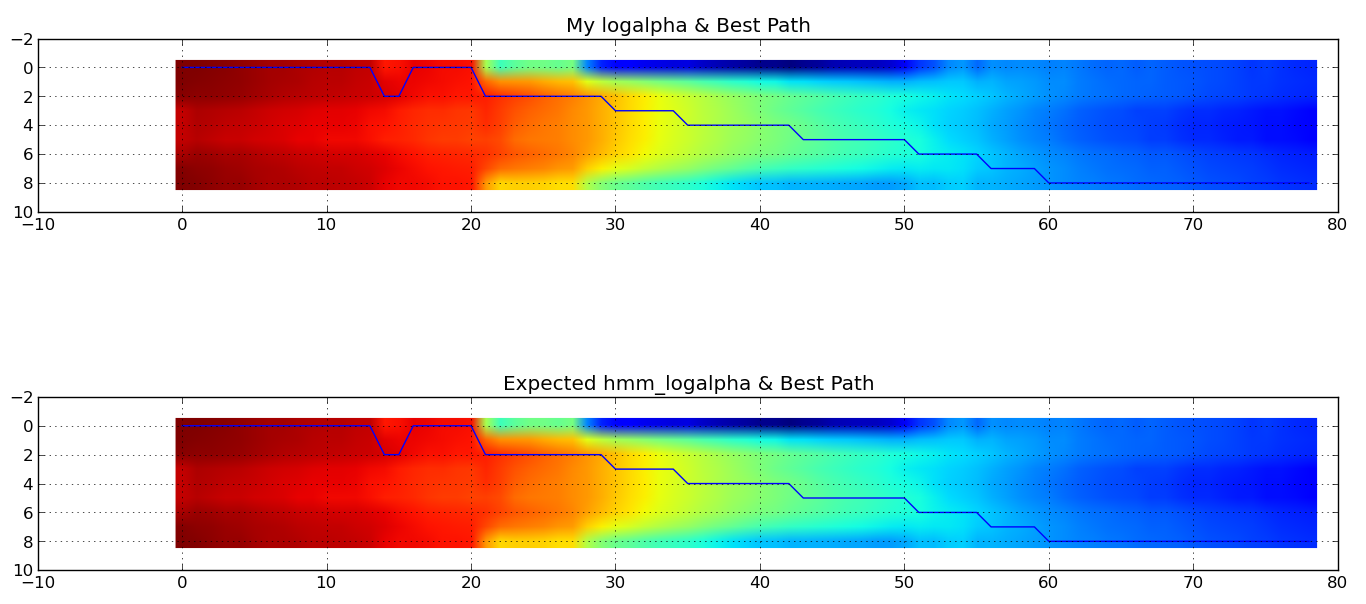
\includegraphics[scale=0.4]{../logalpha.png}
\caption{Alpha probabilities and most probable path}
\label{fig:logalpha}
\end{figure}

After performing one final classification, choosing for every utterance the digit of the model with the most probable path, we get the results shown in Table \ref{tab:Viterbi_class}. This classification is as successful as the one shown in Table \ref{tab:HMM_class}, for which we used the sequence's likelihood for every model based on the forward probabilities. In both cases we have only one misclassification (it occurs for the same utterance).

I believe that this similarity is to be expected. That is because, when calculating the Viterbi probabilities, we choose only the most probable state of every time-step in order to calculate the next time-step's probabilities, whereas in the forward algorithm, we combine all possible states for every time-step. This results in different ultimate likelihoods that are, in a way, scaled. But the ``ranking'' final probability of every model compared to all the others should remain the same. This means, that even though the Viterbi algorithm doesn't produce a likelihood of the observation sequence itself, but produces the likelihood of the most probable state sequence that could produce the observation sequence, nevertheless the likelihood of the most probable state sequence should be higher for the model that was trained on the same digit as the one in the utterance that we have to recognize.

\begin{table}[!ht]
\begin{center}
\footnotesize
\caption{Actual digit of an utterance and the classification using the Viterbi probability} \label{tab:Viterbi_class}
    \begin{tabular}{||c|c||c|c||}
    \hline
    Act. & Class. & Act. & Class. \\
    \hline
    o & o & o & z \\
    o & o & o & o \\
    z & z & z & z \\
    z & z & z & z \\
    1 & 1 & 1 & 1 \\
    1 & 1 & 1 & 1 \\
    2 & 2 & 2 & 2 \\
    2 & 2 & 2 & 2 \\
    3 & 3 & 3 & 3 \\
    3 & 3 & 3 & 3 \\
    4 & 4 & 4 & 4 \\
    4 & 4 & 4 & 4 \\
    5 & 5 & 5 & 5 \\
    5 & 5 & 5 & 5 \\
    6 & 6 & 6 & 6 \\
    6 & 6 & 6 & 6 \\
    7 & 7 & 7 & 7 \\
    7 & 7 & 7 & 7 \\
    8 & 8 & 8 & 8 \\
    8 & 8 & 8 & 8 \\
    9 & 9 & 9 & 9 \\
    9 & 9 & 9 & 9 \\
    \hline
    \end{tabular}
    \end{center}
\end{table}


\end{document}